\section{Proof}
The authors of \cite{kanj} use $LDel^{(2)}(U) $ as the underlying subgraph of the Modified Yao Step.
$LDel^{(2)}(U) $ is defined as the union of the two  subgraph of U in which the circumcircle of every triangle does not contain a 2-hop-neighbor of the nodes which create the triangle and the Gabriel-graph.
However, it is not known whether $LDel^{(2)}(U) $ can be constructed reactively.
At this point I want to introduce the \emph{Partial Delaunay Triangulation (PDT)} \cite{pdt} which might be a valid replacement.
The following part of this work will examine the possibility of this replacement.

At first, note that the style of this proof is adapted from \cite{kanj}.\\
Let U be the Unit Disk Graph of the Euclidean Graph of a Node Set S.
In a style similar to the definition of $LDel^{(2)}(U) $ from \cite{kanj}, we define the Partial Delaunay Triangulation as follows:
\begin{definition}
\label{emptycircle}
An edge XY of U is contained in the PDT graph if and only if there exists a circle trough X and Y whose interior contains no point of U that is a 2-hop neighbor of X or Y.
\end{definition}
\begin{proof}
This can be verified since the original PTD-Definition from \cite{pdt} is defined like above, except that the circle must not contain \emph{any} nodes of U. 
If this region contains no nodes at all, it cannot contain nodes which are 2-hop-neighbors of X or Y either.  
\end{proof}

Additionally, the following Delaunay Graph property is being used:
\begin{lemma}
\label{emptyregion}
If CA and CB are edges of the PDT Graph then the region of $(O)=\bigcirc{ABC} $ subtended by chord  CA and away from B and the region of $(O) $ subtended by chord CB and away from A contain no points that are two hop neighbours of A, B and C.
\end{lemma}


See Figure \ref{fig:empty_region} for a graphical illustration of the above lemma.
This property also holds true for PDT.

\begin{proof}
Since $CA $ is a PDT edge there is a circle $\bigcirc{c_1} $ with C and A on it's border which does not contain any node (so non two-hop-neighbour of C or A, either) of U.
Suppose we take another third Point d, which is not in the Set U, to identify $\bigcirc{c_1} $.
No matter where the third point d of this circle is, the region, in the following named $R_1 $, of $\bigcirc{ABC} $ delimited by chord $CA $ away from B is always contained completely in $\bigcirc{c_1} $ and, therefore, empty.
The next part proofs this proposition.
By symmetry of circles it is sufficient to put d on a line  $l $ which is defined as the perpendicular bisector of $CA $.
Let $\alpha<\pi $ be the smaller angle in $\angle{AdC} $.
If d moves on the line $l $ the angle $\alpha $ changes.   
Let $\beta >0$ be the value of alpha, when $B $ is on the border of circle $\bigcirc{c_1} $.
Let d start at degree $\alpha = \pi-\epsilon $ for $\epsilon $  arbitrarily small.
Since d is continuous in the interval $[\beta,\pi[ $, every possible circle is covered:
\begin{itemize}
\item If $\alpha $ is barely equal to $\pi $, d is located at the nearest position to edge $CA $ on $l $.
\item If $\alpha=\beta $ is satisfied, $B $ is on the border of $\bigcirc{c_1} $.
\item If $\alpha <\beta $ is satisfied, $B $ is contained in the circle and hence, this is not a valid circle.
\end{itemize}
Suppose $c_1 $ is the Gabriel circle ($\alpha=\frac{\pi}{2} $).
Then $R_1 $ is contained in $c_1 $. 
If $\alpha $ is a value in $[\frac{\pi}{2},\pi[ $ the circle $c_1 $ expands on the side of $CA $ on which $R_1 $ is located which means that $R_1 $ must still be inside $c_1 $.
If $alpha $ is a value in $]\frac{\pi}{2},\beta[ $ the circle shrinks on the side of $CA $ on which $R_1 $ is located.
Since $R_1 $ was created from $\bigcirc{ABC} $ and at $\alpha=\beta $ these two circles $\bigcirc{ABC} $ and $c_1 $ are identical, $R_1 $ must reside in $c_1 $.    
Therefore, it does not matter which circle of them is the PDT-circle $c_1 $, since all circles cover the region $R_1 $.

\end{proof} 



We need to show that there is a path from $A $ to $B $ which has length at most of $(1+2\pi (k*\cos{\frac{\pi}{k}})^{-1})|CB| $ for integer $ k \geq 14 $. 
Keil and Gutwin \cite{keil} proved the existence of a path between the Points $A $ and $B $ and showed that the length of this path is delimited by the length of the arc from $A $ to $B $ on the circle $\bigcirc{ABC} $.
The only precondition is that lemma \ref{emptyregion} holds (which it does).
This path is called the \emph{outward Path}.
\begin{figure}[h!]
\centering
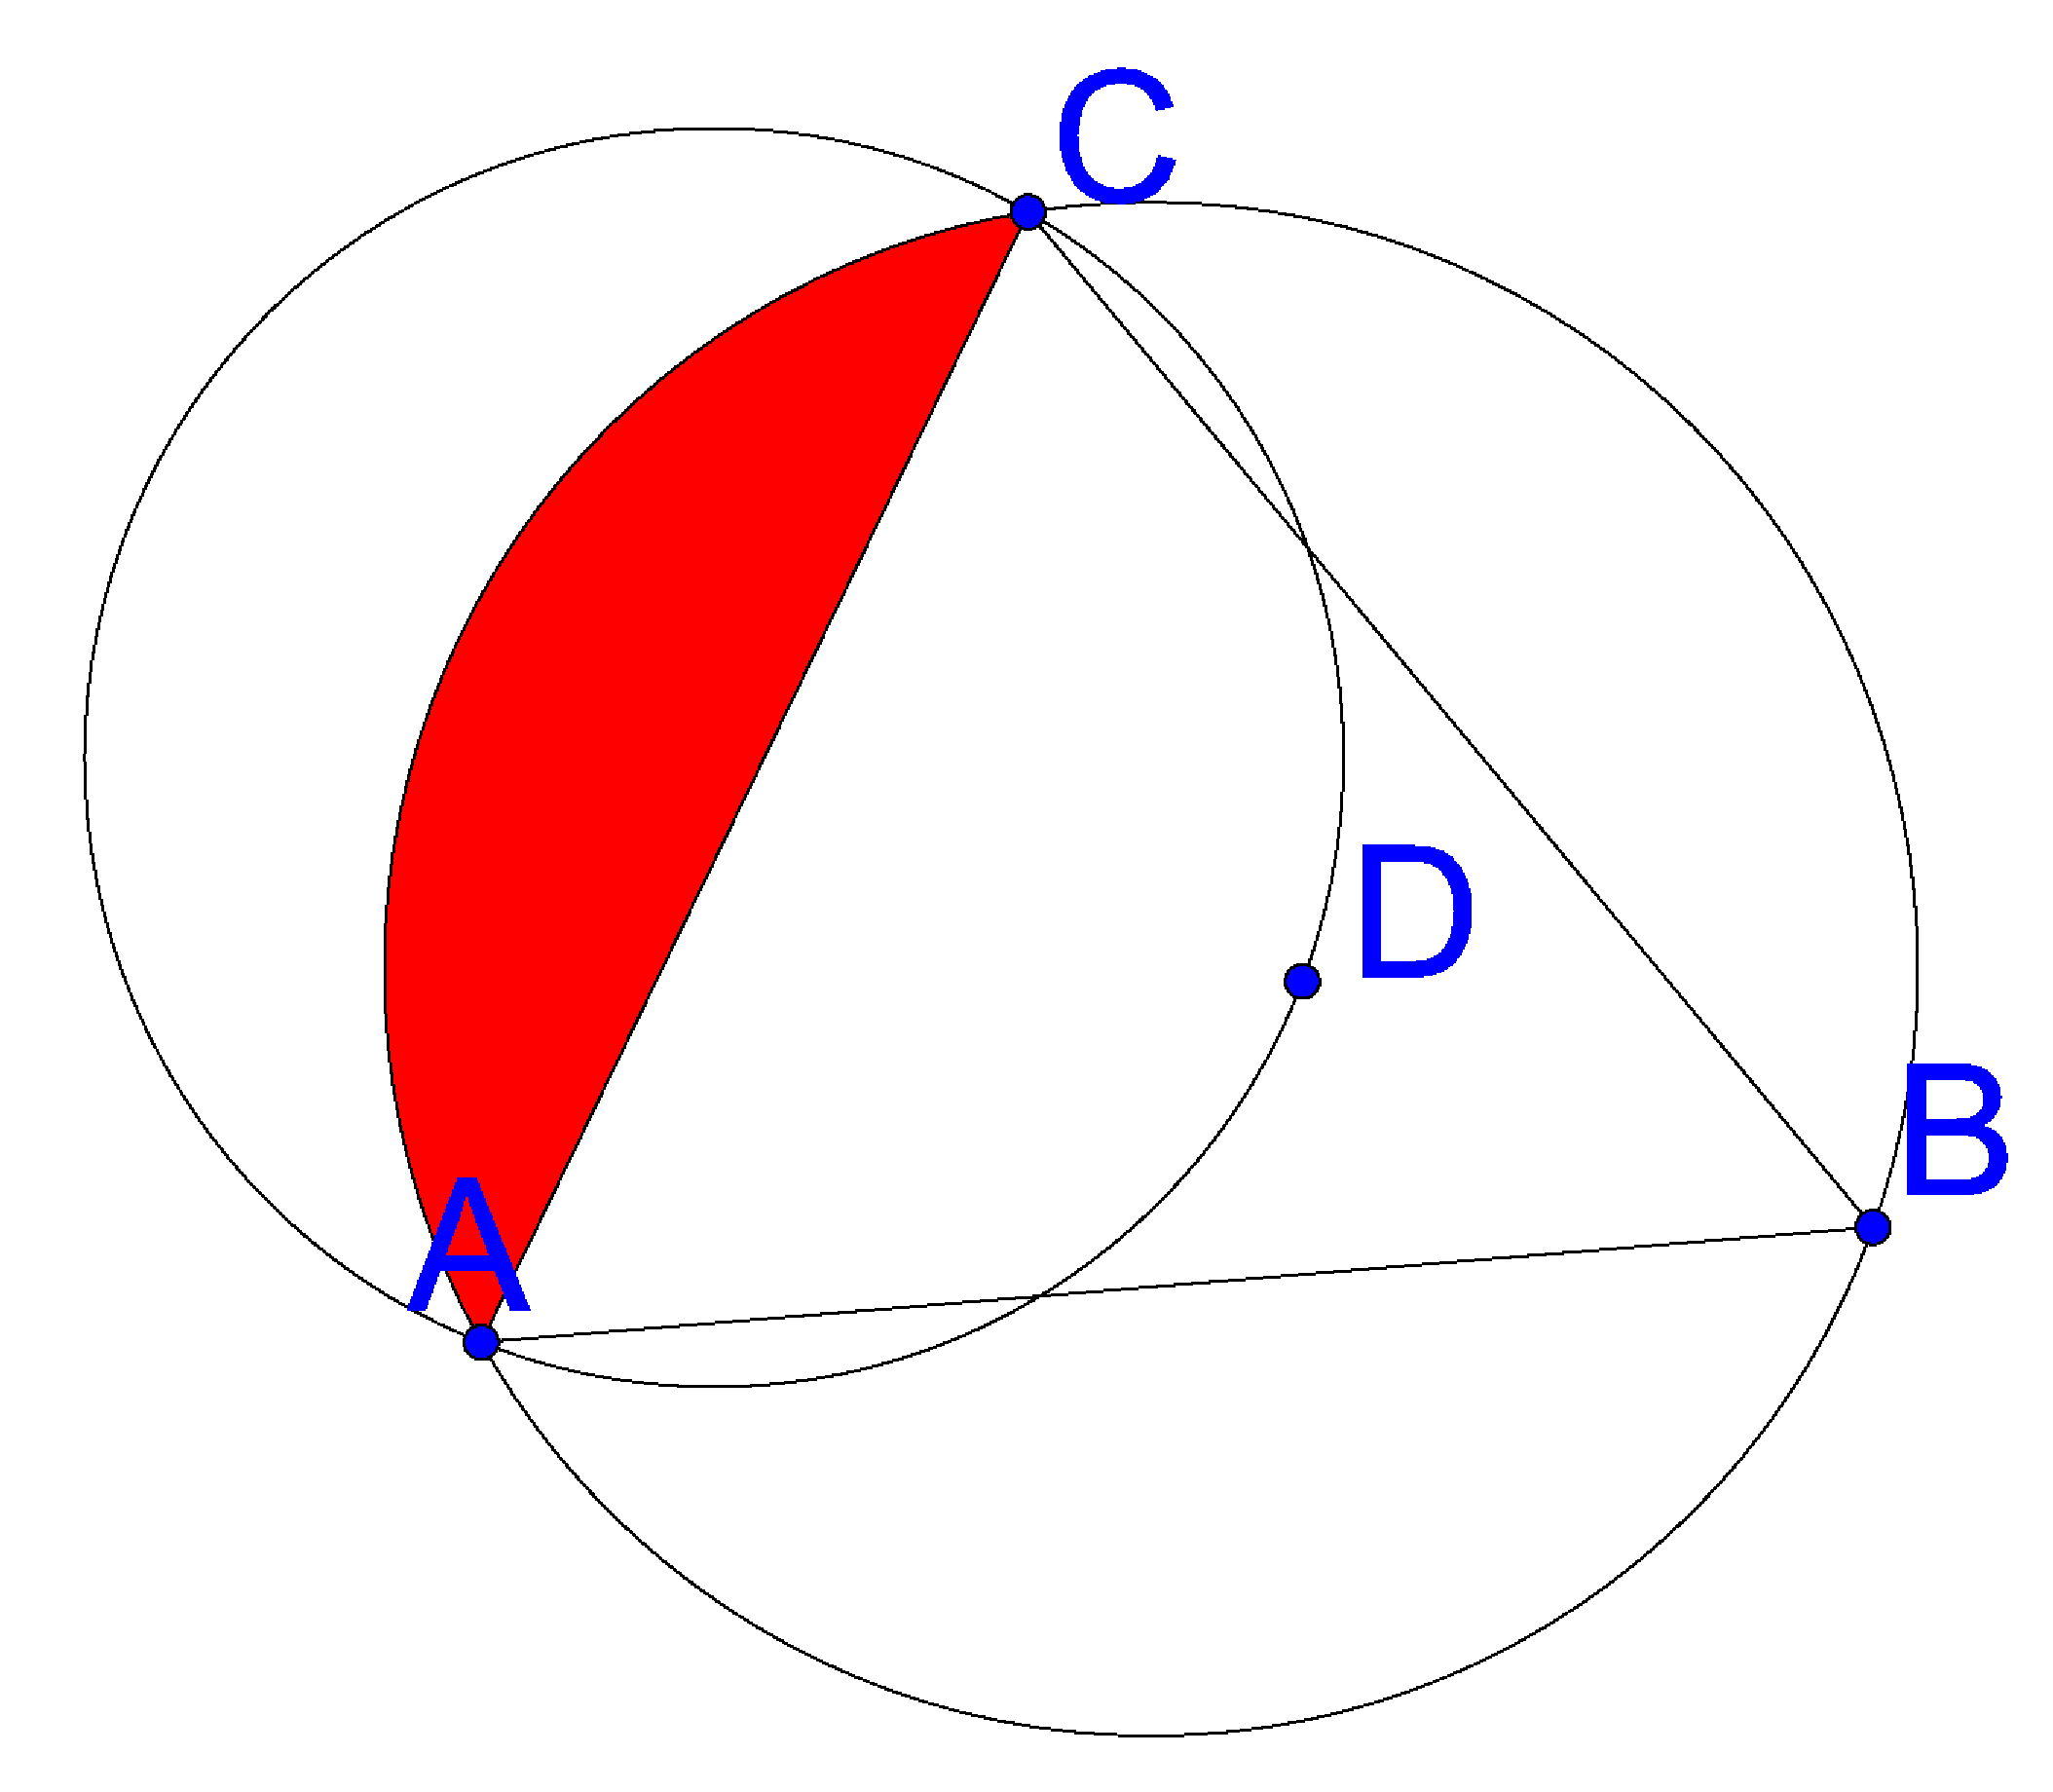
\includegraphics[width=0.2\linewidth]{eps/noPointinRegion.eps}
\caption{The red marked region contains no Points of G because it is always contained in $\bigcirc{ACD} $ which must be empty by definition.}
\label{fig:empty_region}
\end{figure}

This proof is divided into two cases: when $\triangle{ABC} $ contains nodes of G and when this triangle is devoid of any nodes of G.
The outward path connects $A $ and $B $ when no other points of G are inside $\triangle{ABC} $
We must proof the following proposition:

\begin{prop}
In every recursive step of the outward path construction described above, if $M_p $ is an intermediate point with respect to a pair of points $(M_i, M_j) $, then:
\begin{enumerate}
\item there is a circle passing through C and $M_p $ that contains no point of G, and
\item circles $\bigcirc{CM_iM_p} $ and $\bigcirc{CM_jM_p} $ contain no points of G, except, possibly, in the region subtended by chords $M_iM_p $ and $M_pM_j $, respectively, away from C.
\end{enumerate}
\end{prop}

\begin{proof}

\end{proof}

\begin{enumerate}
\item $|CA| + \sum\nolimits_{i=0}^{r-1} |M_iM_{i+1}| \leq (1+2\pi (k*\cos{\frac{\pi}{k}})^{-1})|CB| $
\item There is no edge in G between any pair $M_i $ and $M_j $ lying in the closed region delimited by CA, CB and the edges of p, for any i and j satisfying $0 \leq i < j-1 \leq r $ 
\item $\angle{M_{i-1}M_iM_{i+1}} > \frac{k-2}{k}\pi $, for $i=1, ..., r-1 $ 
\item $\angle{CAM_1} \geq \frac{\pi}{2}-\frac{\pi}{k} $
\end{enumerate}

